\documentclass[../main.tex]{subfiles}
\begin{document}
\chapter{Systemintegration} \label{Chap:Systemintegration}
Til sidst samles alle underdelene af projektet og der sørges for at de spiller sammen som forventet. Figur \ref{fig: Samlet Setup} viser hele systemet efter det blev godkendt af hjælpelæreren. Videoen i Appendiks \ref{subsection:System test} viser systemet køre, hvor der bliver skiftevist blokeret og ikke blokeret for sollyset på solcellen. Når solen er blokeret kan det ses, og høres, at motoren starter. Når der ikke blokeres, stopper motoren helt, og alt energien kommer fra solcellen. Dette opfylder dermed både Krav 11 og 16 i kravspecifikationen. 

\begin{figure}[H]
      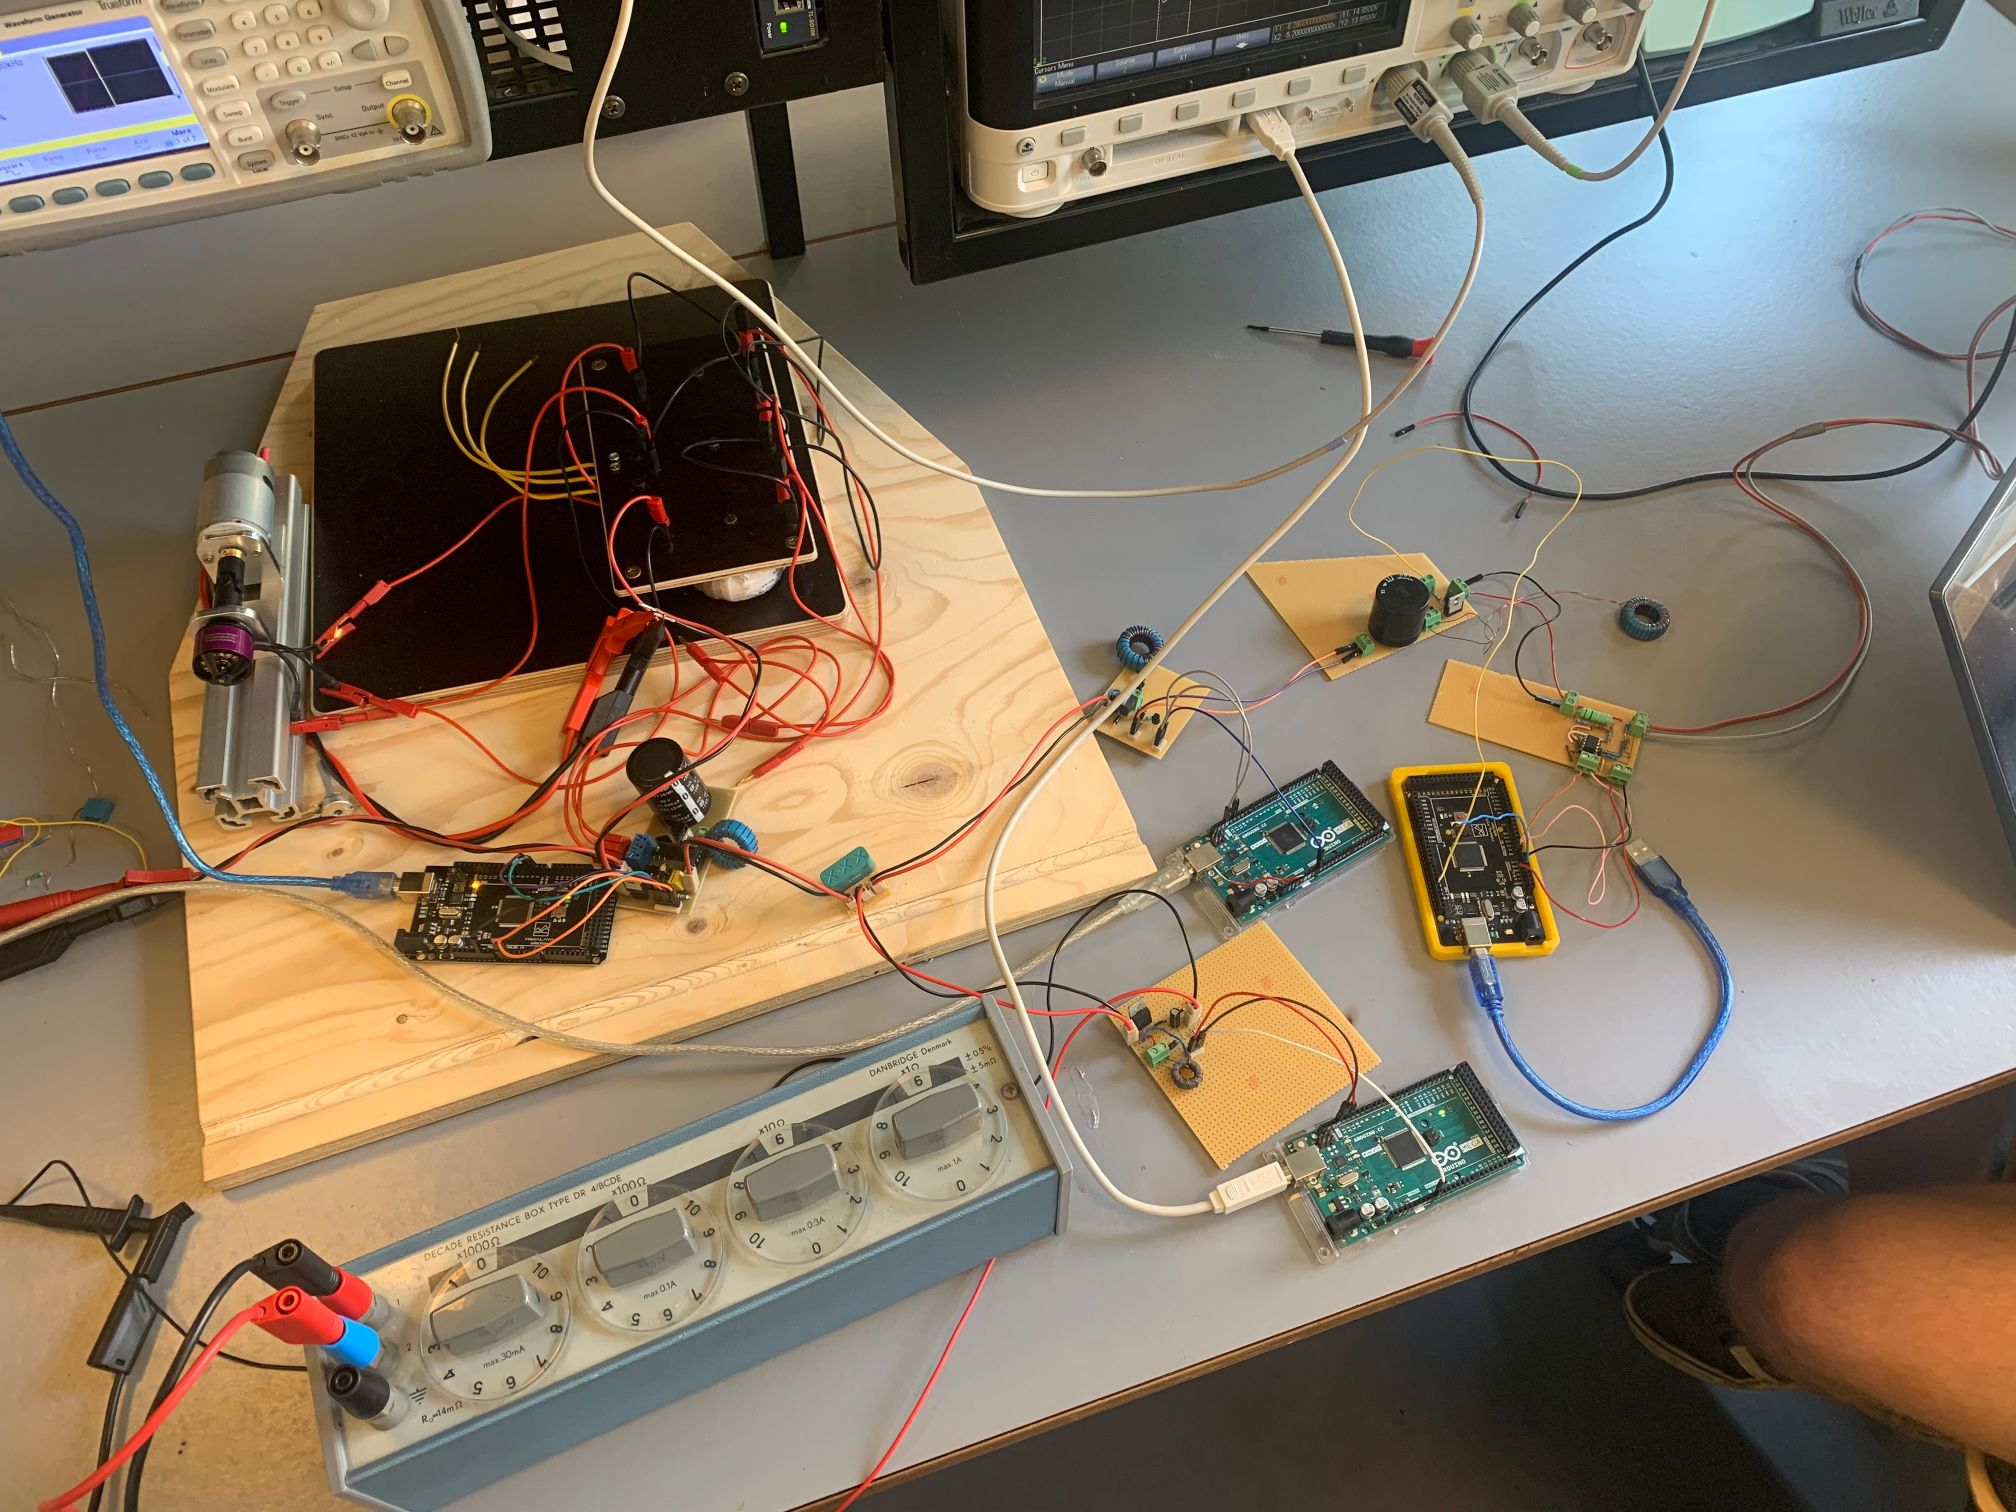
\includegraphics[width=\textwidth]{Dokumentation/Pictures/Total Setup.jpg}
     \caption{Samlet Setup}
     \label{fig: Samlet Setup}
     \end{figure}

\end{document}